\begin{figure}
    \centering
    \adjustbox{valign=t}{
        \begin{minipage}{0.68\linewidth}
            \begin{minipage}{\linewidth}
                {
                    \hspace{4em}
                    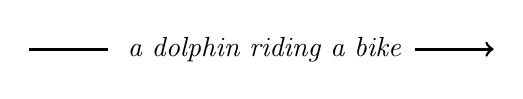
\begin{tikzpicture}
                        \draw[-, line width=1pt] (0,0) -- (1,0);
                        \node at (3,0) {\emph{a dolphin riding a bike}}; 
                        \draw[->, line width=1pt] (4.9,0) -- (5.9,0);
                    \end{tikzpicture} \\
                }
                \lfbox[
                    border-width=2pt,
                    padding-top=0pt,
                    padding-bottom=0pt,
                    padding-left=-2.6pt,
                    padding-right=-2.5pt,
                ]{
                    \includegraphics*[width=0.2\linewidth]{vlm/dolphin_bike/0.jpg}
                    \hspace{-0.7em}
                    
\includegraphics[width=0.2\linewidth]{vlm/dolphin_bike/1.jpg}
                    \hspace{-0.7em}
                    \includegraphics*[width=0.2\linewidth]{vlm/dolphin_bike/2.jpg}
                    \hspace{-0.7em}
                    \includegraphics*[width=0.2\linewidth]{vlm/dolphin_bike/3.jpg}
                    \hspace{-0.7em}
                    \includegraphics*[width=0.2\linewidth]{vlm/dolphin_bike/5.jpg}
                }
            \end{minipage}
            \vspace{0em} \\
            \begin{minipage}{\linewidth}
                {
                    \hspace{4em}
                    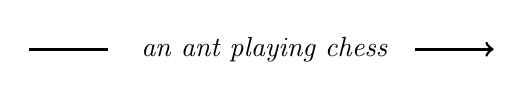
\begin{tikzpicture}
                        \draw[-, line width=1pt] (0,0) -- (1,0);
                        \node at (3,0) {\emph{an ant playing chess}}; 
                        \draw[->, line width=1pt] (4.9,0) -- (5.9,0);
                    \end{tikzpicture} \\
                }
                \lfbox[
                    border-width=2pt,
                    padding-top=0pt,
                    padding-bottom=0pt,
                    padding-left=-2.6pt,
                    padding-right=-2.5pt,
                ]{
                    \includegraphics*[width=0.2\linewidth]{vlm/ant_chess/0.jpg}
                    \hspace{-0.7em}
                    
\includegraphics[width=0.2\linewidth]{vlm/ant_chess/1.jpg}
                    \hspace{-0.7em}
                    \includegraphics*[width=0.2\linewidth]{vlm/ant_chess/3.jpg}
                    \hspace{-0.7em}
                    \includegraphics*[width=0.2\linewidth]{vlm/ant_chess/4.jpg}
                    \hspace{-0.7em}
                    \includegraphics*[width=0.2\linewidth]{vlm/ant_chess/5.jpg}
                }
            \end{minipage}
            \vspace{0em} \\
            \begin{minipage}{\linewidth}
                {
                    \hspace{4em}
                    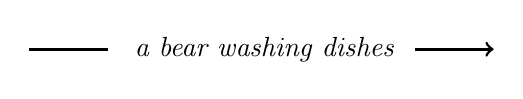
\begin{tikzpicture}
                        \draw[-, line width=1pt] (0,0) -- (1,0);
                        \node at (3,0) {\emph{a bear washing dishes}}; 
                        \draw[->, line width=1pt] (4.9,0) -- (5.9,0);
                    \end{tikzpicture} \\
                }
                \lfbox[
                    border-width=2pt,
                    padding-top=0pt,
                    padding-bottom=0pt,
                    padding-left=-2.6pt,
                    padding-right=-2.5pt,
                ]{
                    \includegraphics*[width=0.2\linewidth]{vlm/bear_dishes/0.jpg}
                    \hspace{-0.7em}
                    \includegraphics*[width=0.2\linewidth]{vlm/bear_dishes/2.jpg}
                    \hspace{-0.7em}
                    \includegraphics*[width=0.2\linewidth]{vlm/bear_dishes/3.jpg}
                    \hspace{-0.7em}
                    \includegraphics*[width=0.2\linewidth]{vlm/bear_dishes/4.jpg}
                    \hspace{-0.7em}
                    \includegraphics*[width=0.2\linewidth]{vlm/bear_dishes/5.jpg}
                }
            \end{minipage}
        \end{minipage}
    }
    \hspace{-0.5em}
    \adjustbox{valign=t}{
        \begin{minipage}{0.29\linewidth}
            ~\vspace{1.5em} \\
            
\includegraphics[width=\linewidth]{vlm/plot.pdf} \\
            \vspace{-0.5em}\\
            \footnotesize
            ~\hspace*{3em}\raisebox{0.2em}{\color{bike}\rule{1.5em}{0.15em}}
                ~\emph{\ldots riding a bike} \\
            ~\hspace*{3em}\raisebox{0.2em}{\color{chess}\rule{1.5em}{0.15em}}
                ~\emph{\ldots playing chess} \\
            ~\hspace*{3em}\raisebox{0.2em}{\color{dishes}\rule{1.5em}{0.15em}}
                ~\emph{\ldots washing dishes}
        \end{minipage}
    }
    \vspace{0.0em}\\
    \caption{
        \textbf{(Prompt alignment)}
        \textbf{(L)}
        Progression of samples for the same prompt and random seed over the course of training.
        The images become significantly more faithful to the prompt.
        The samples also adopt a cartoon-like style, which we hypothesize is because the prompts are more likely depicted as illustrations than realistic photographs in the pretraining distribution.
        \textbf{(R)}
        Quantitative improvement of prompt alignment.
        Each thick line is the average score for an activity, while the faint lines show average scores for a few randomly selected individual prompts.
    }
    \label{fig:vlm_progression}
    \vspace{-1.2em}
\end{figure}

